\subsection{Structure}

\begin{figure}[H]
    \centering
    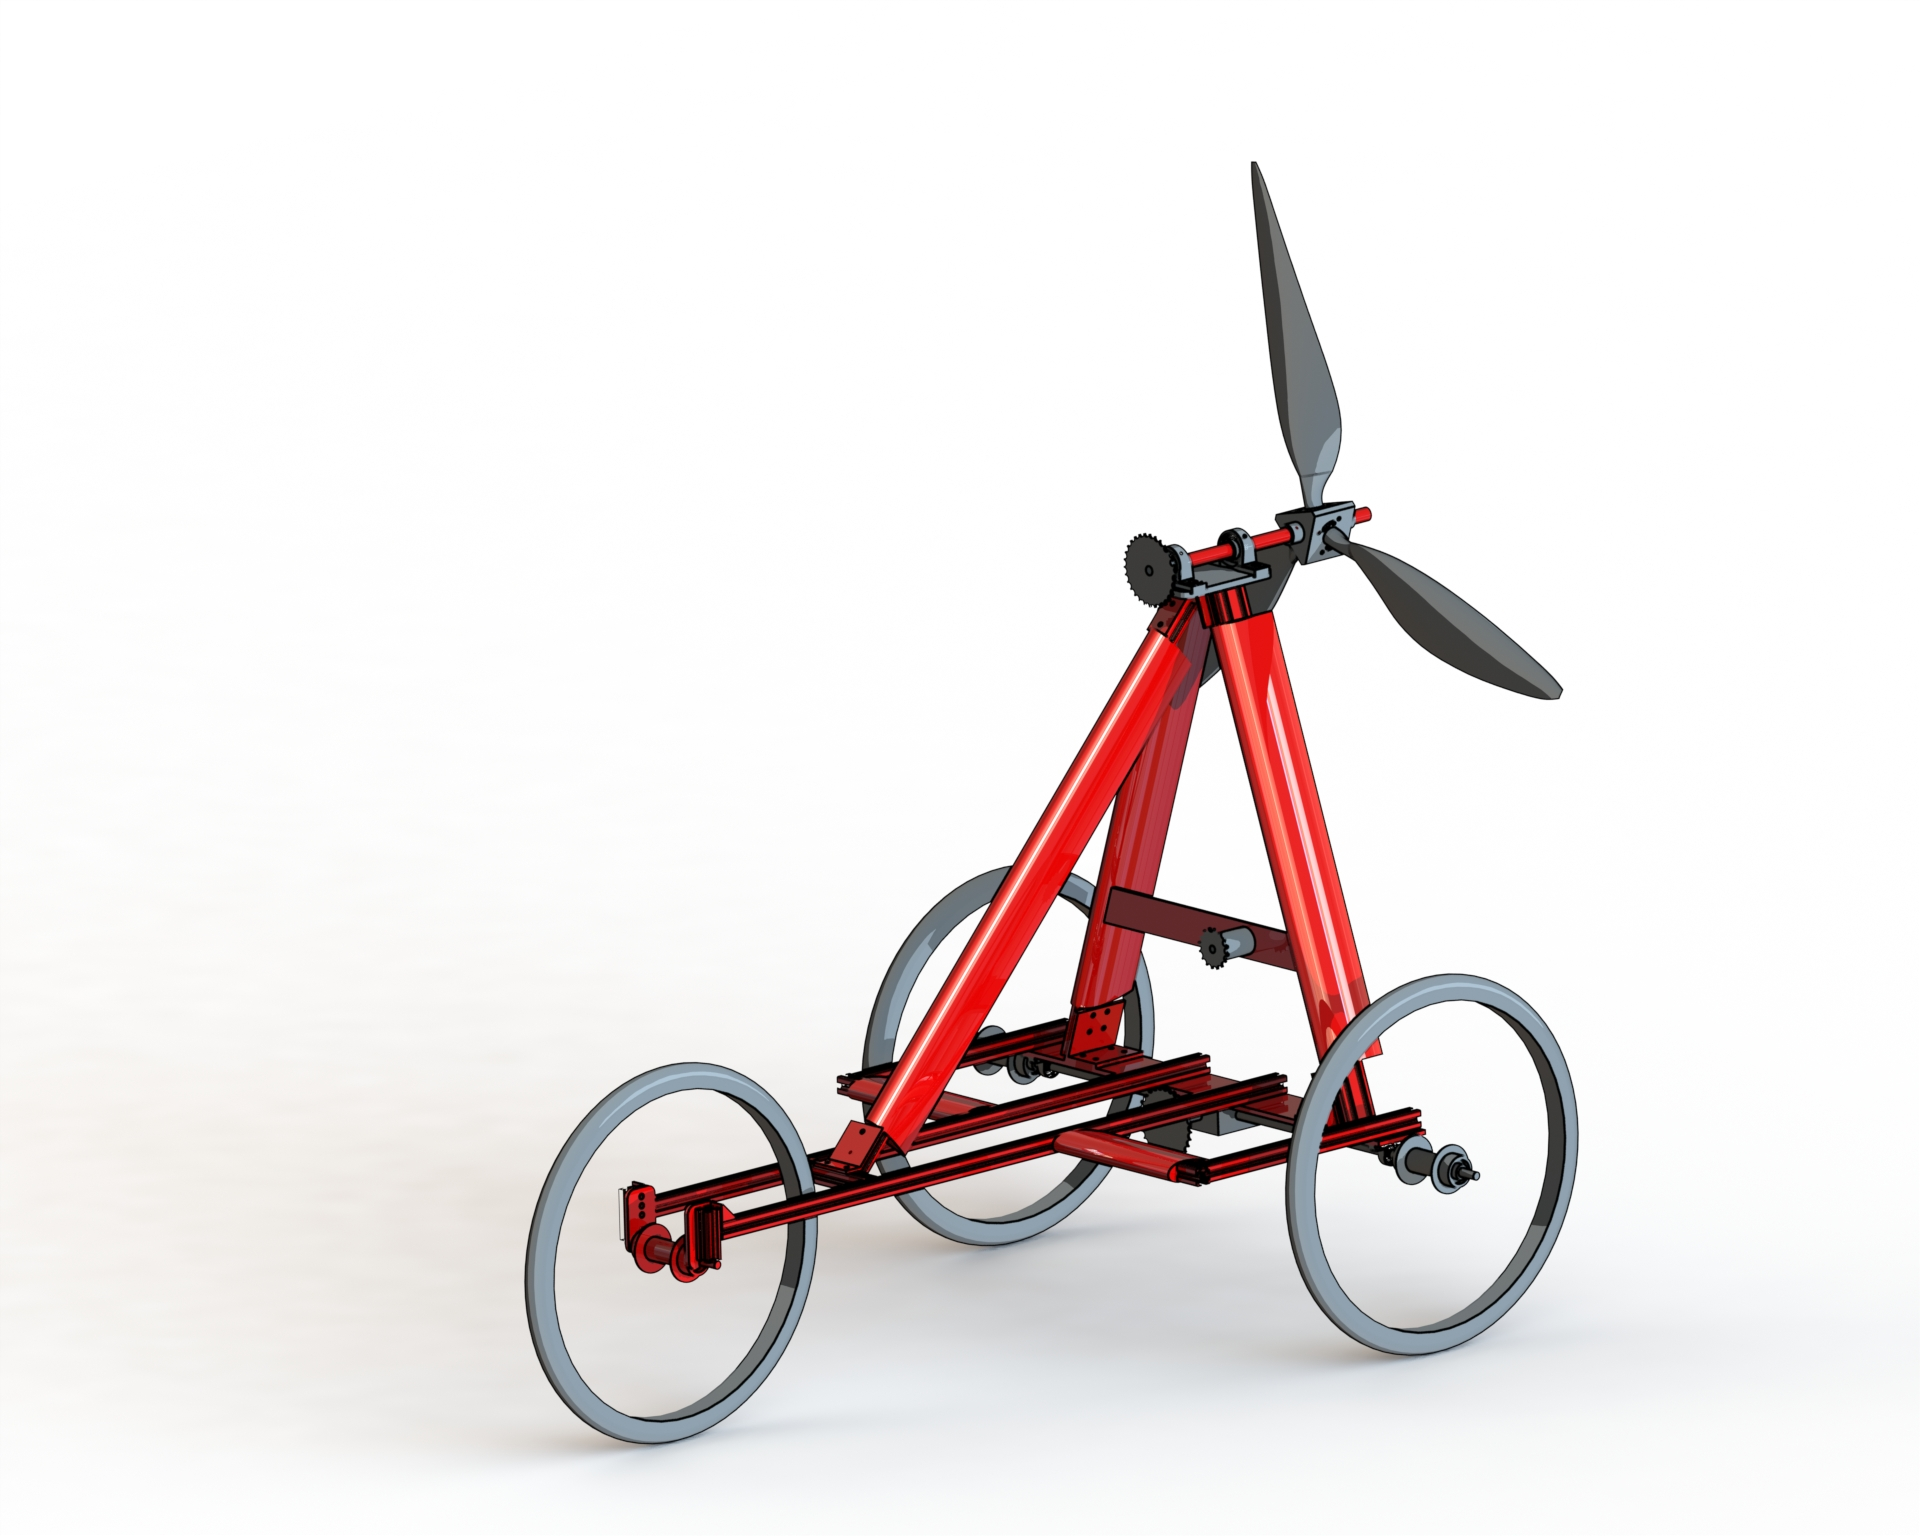
\includegraphics[width = 0.5\linewidth]{images/renders/structure.JPG}
    \caption{Structure of the prototype}
    \label{fig:structrender}
\end{figure}

The overall structure is a construction weighing 11kg, excluding the propeller (Figure \ref{fig:structrender}). It is comprised of mainly aluminium profile 20x20 mm and 20x40 mm beams, aluminium plates, all bolted together and connected to the drivetrain, propeller shaft, and wheels. The structure is a simple, stiff design which effectively facilitates testing in the wind tunnel as per the project requirements. The vehicle length is 1137 mm, the height including the top sprocket (propeller dismounted) is 820 mm, and the maximum width at the rear is 800 mm. The vehicle is lightweight due to the use of aluminium parts and by efficient use of material.


\subsection{Drivetrain and transmission}

\begin{figure}[H]
    \centering
    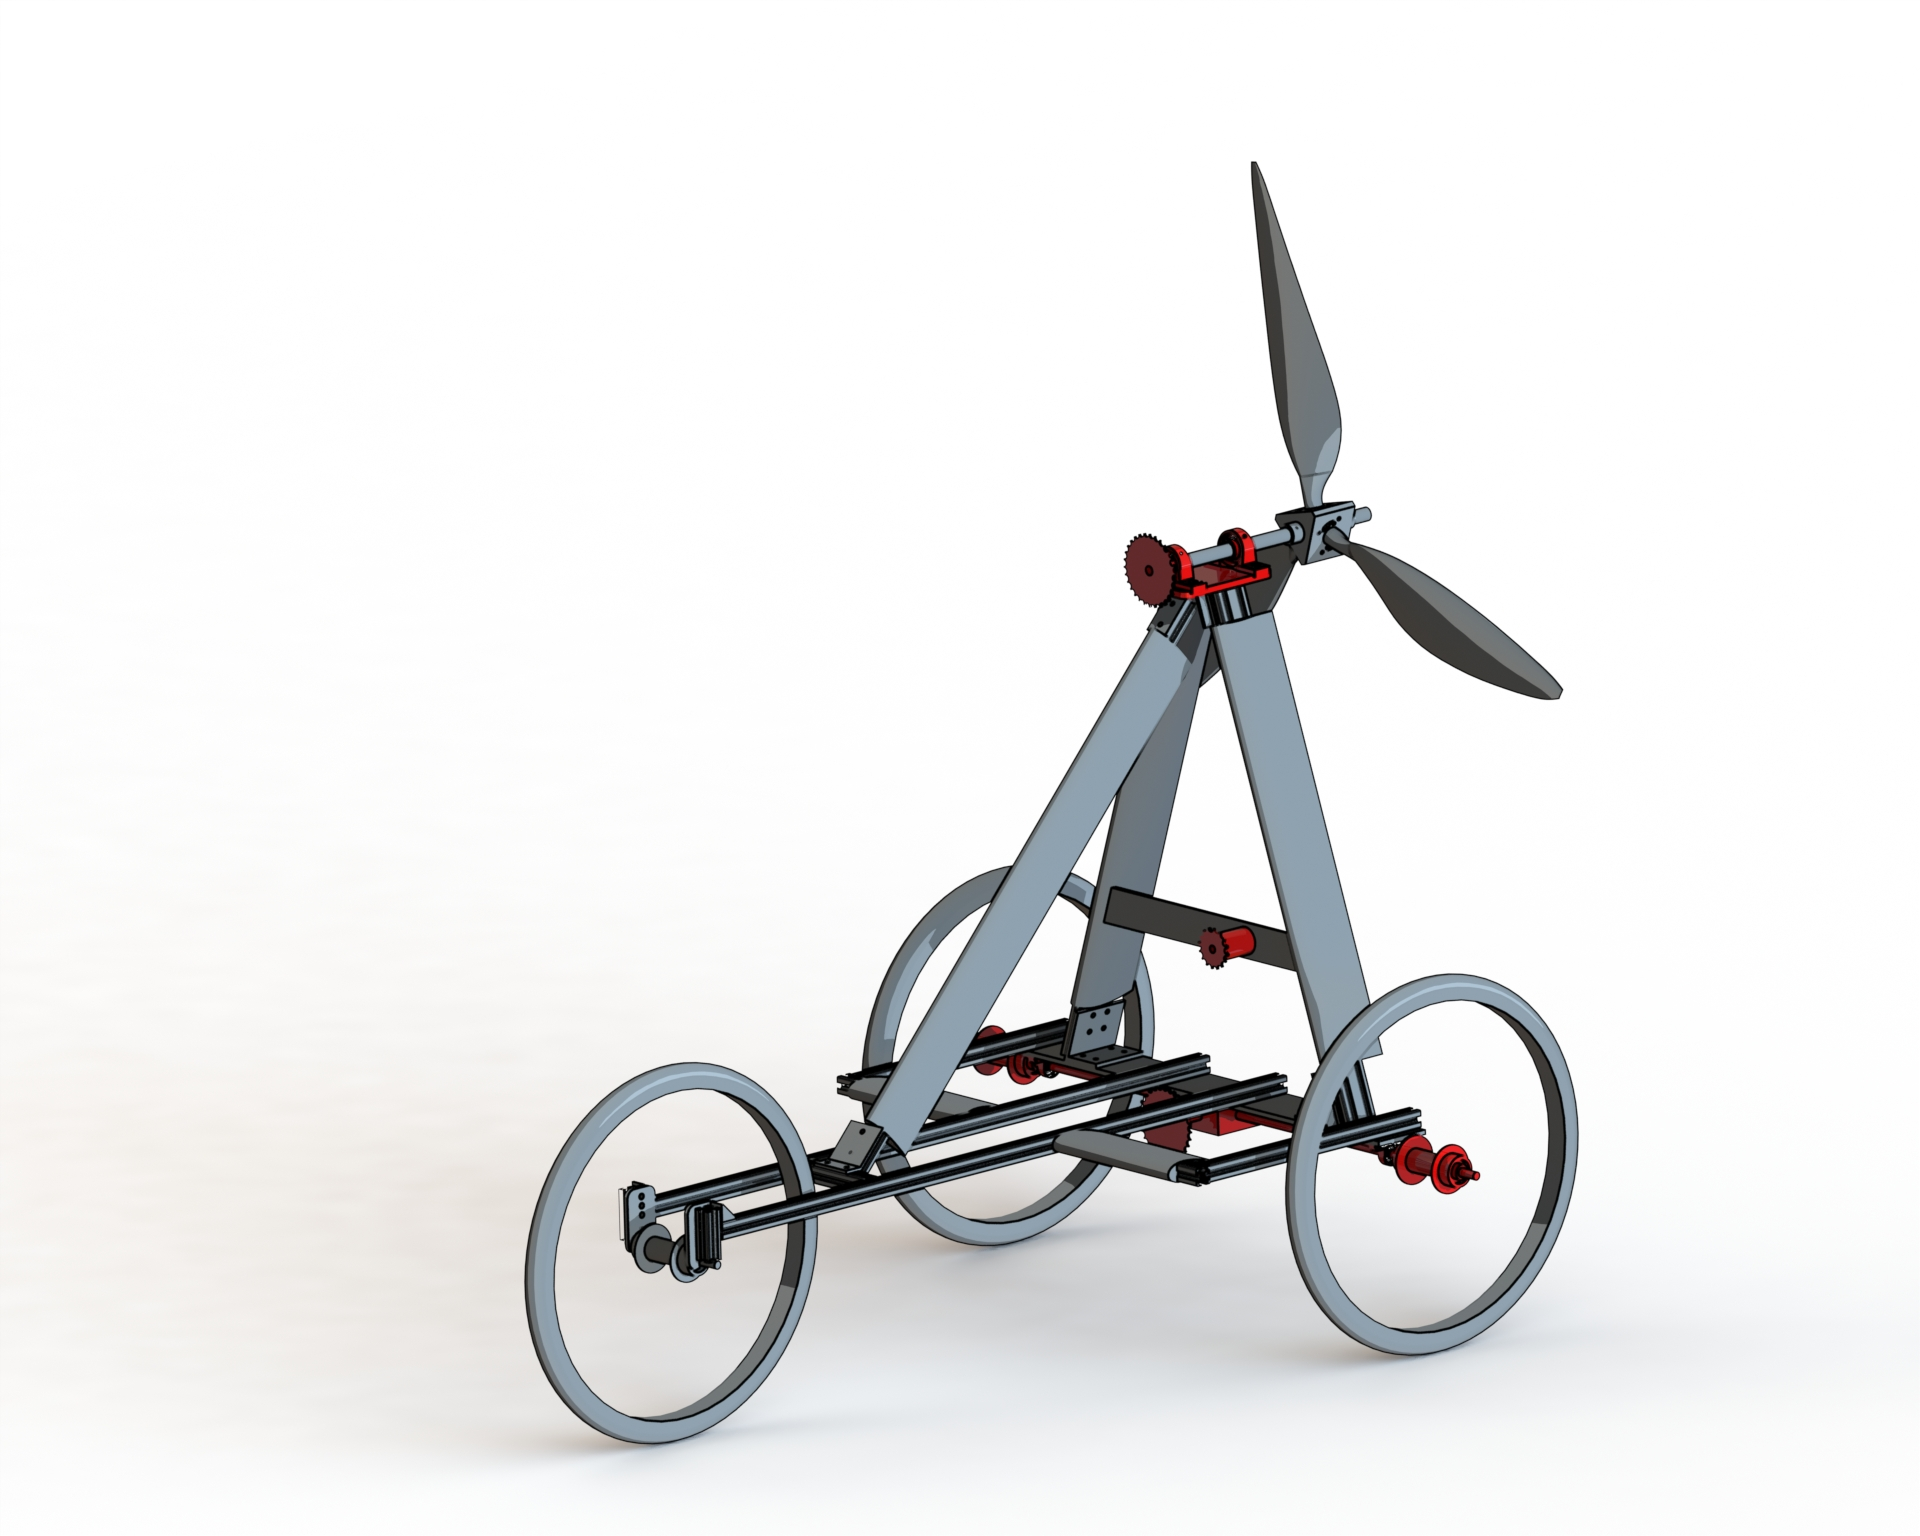
\includegraphics[width = 0.5\linewidth]{images/renders/drivetrain.JPG}
    \caption{Transmission of the prototype}
    \label{fig:transmirender}
\end{figure}

The final transmission system  (Figure \ref{fig:transmirender}) consists of an axle shaft connected to a chain through a right-angle gearbox. This chain drives the propeller shaft situated on top of the vehicle. The chain is kept in tension by a chain tensioner mechanism which can be adjusted based on the needs. The gear ratio between the prop-shaft sprocket and driven sprocket is 1:1, both 30 tooth, with an 8mm pitch chain running between them. The chain tensioner sprocket used is 24 tooth, running on a bearing to minimize resistance and mounted to an aluminium plate fixed to the A-frame.

\subsection{Propeller and hub}

\begin{figure}[H]
    \centering
    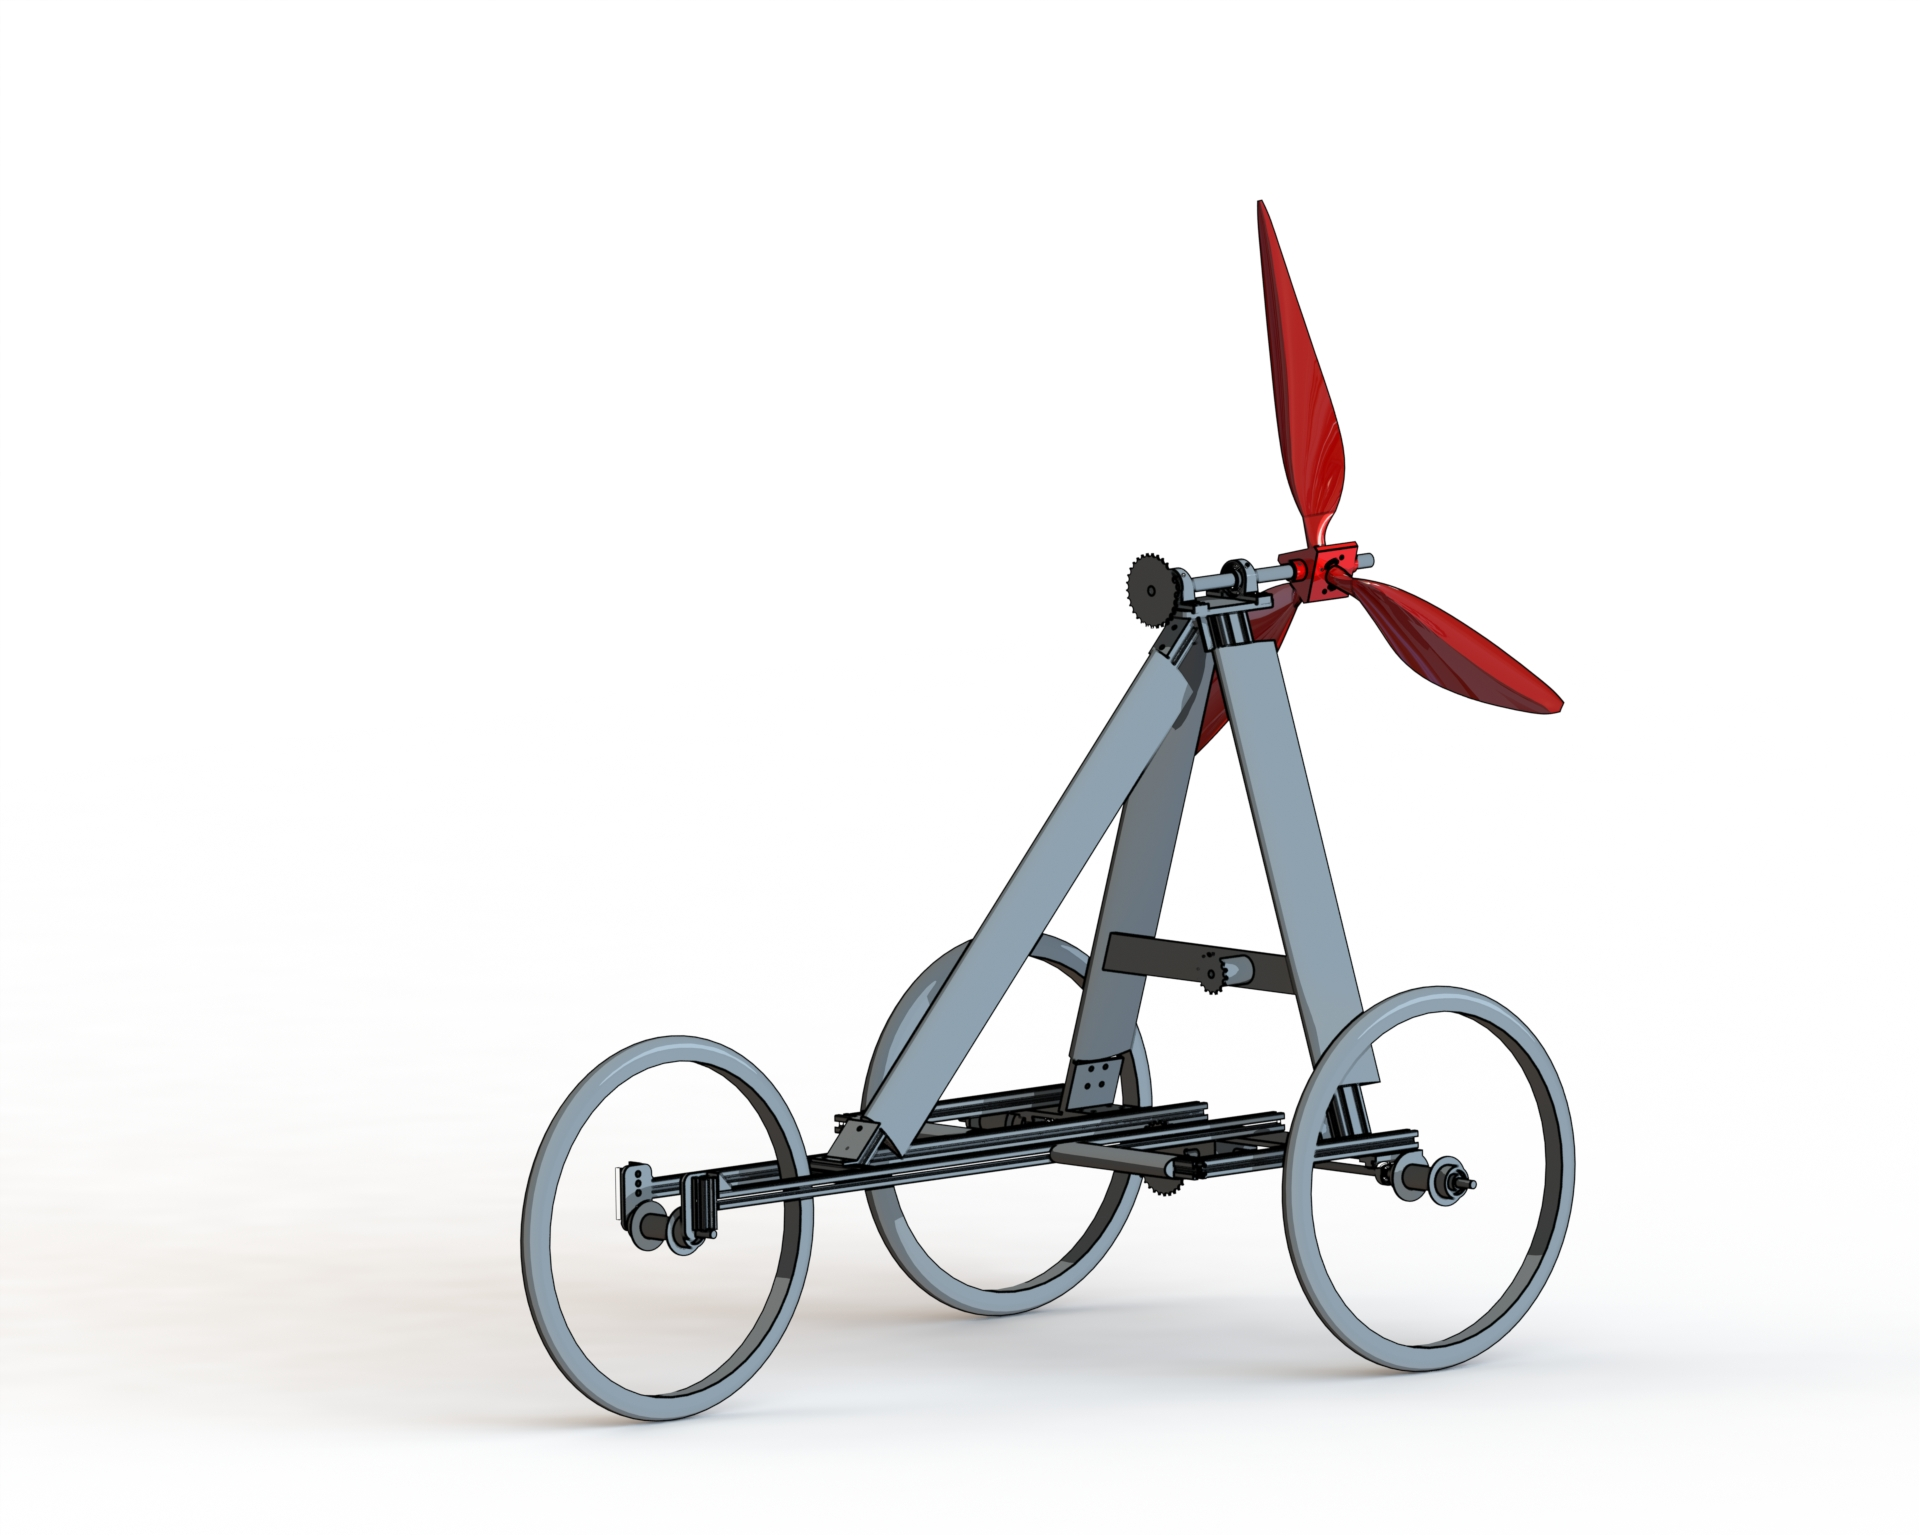
\includegraphics[width = 0.5\linewidth]{images/renders/prop.JPG}
    \caption{Propeller and hub of the prototype}
    \label{fig:proprender}
\end{figure}


The final propeller (Figure \ref{fig:proprender}) is composed of 3 blades featuring the ability to vary the pitch angle by $20^\circ$ in both directions. It is 780 mm in diameter. The blades used a NACA 6412 profile along the entire PLA 3D printed mid-section. The blades can be swapped out for different ones within minutes with the highly modular design. This also implies that transportation of the propeller is facilitated. The hub has a diameter of 71 mm and is designed to fit on a 16 mm shaft.

